\documentclass[12pt]{extreport}

\usepackage[top=1in,bottom=1.25in,left=1.5in,right=1in]{geometry}
\usepackage{array}
\usepackage{float}
\usepackage{amsfonts}
\usepackage{graphicx}
\usepackage{wrapfig}
\usepackage{setspace}
\usepackage{pgf}
\usepackage{tikz}
\usetikzlibrary{arrows,automata}
\usetikzlibrary{shapes.geometric,fit}
\usepackage{titlesec}
\usepackage{tocloft}
\usepackage{longtable}
\usepackage{lscape}
\usepackage[nottoc]{tocbibind}
\usepackage{fancyhdr}
\usepackage{inputenc}
\usepackage{enumitem}
\usepackage{titlesec}
\usepackage{fixltx2e}
\titleformat{\chapter}[display]
{\normalfont\huge\bfseries\centering}{\chaptertitlename\ \thechapter}{14pt}{\Huge}
% Define block styles
\tikzstyle{decision} = [diamond, draw, fill=blue!20, 
    text width=4.5em, text badly centered, node distance=3cm, inner sep=0pt]
\tikzstyle{block} = [rectangle, draw, text width=5em, text centered, rounded corners, minimum height=4cm]
\tikzstyle{line} = [draw, -latex']
\tikzstyle{cloud} = [draw, circle, node distance=3cm,
    minimum height=2em]

\renewcommand{\cftaftertoctitle}{\hrulefill}

\renewcommand*\contentsname{CONTENTS}
\renewcommand*{\listfigurename}{LIST OF FIGURES}
\renewcommand*{\listtablename}{LIST OF TABLES}


\setlist[enumerate,1]{label={(\alph*)}}
\setlist[enumerate,2]{label={(\roman*)}}

\newcounter{parnum}
\newcommand{\N}{%
   \noindent\refstepcounter{parnum}%
    \makebox[\parindent][l]{\textbf{\arabic{parnum}.}}}
    
 \setlength{\parindent}{5em}
    
         
 \renewcommand{\arraystretch}{1.2}  
 
\newcolumntype{M}[1]{{\centering\arraybackslash}m{#1}} 

\renewcommand{\cfttoctitlefont}{\hspace*{\fill}\Huge\bfseries}
\renewcommand{\cftaftertoctitle}{\hspace*{\fill}}
\renewcommand{\cftlottitlefont}{\hspace*{\fill}\Huge\bfseries}
\renewcommand{\cftafterlottitle}{\hspace*{\fill}}
\renewcommand{\cftloftitlefont}{\hspace*{\fill}\Huge\bfseries}
\renewcommand{\cftafterloftitle}{\hspace*{\fill}}


\begin{document}
\begin{titlepage}
\begin{titlepage}
\centering


%\end{document}

%\onehalfspacing
\textbf{A PROJECT REPORT ON}\\\vspace{1cm}\large\textbf{"CRIME ANALYSIS AND PREDICTION AS AN APPLICATION OF DATA MINING"}\\\vspace{1cm}

SUBMITTED TO THE SAVITRIBAI PHULE PUNE UNIVERSITY, PUNE
IN THE PARTIAL FULFILLMENT OF THE REQUIREMENTS 
FOR THE AWARD OF THE DEGREE 
\begin{center}

\vspace{1cm} OF\\\vspace{1cm}\textbf{BACHELOR OF ENGINEERING (COMPUTER ENGINEERING) }\\\vspace{1cm}BY\vspace{1cm}\\
{\small{AKSHAY KUMAR SINGH} \hspace{22mm} {\small ROLL NO:12CO057}\\{NEHA PRASAD} \hspace{36.5mm} {\small ROLL NO:12CO042 } \\{NOHIL NARKHEDE} \hspace{29mm} {\small ROLL NO:12CO041 } \\{SIDDHARTH MEHTA} \hspace{26.8mm} {\small ROLL NO:12CO039 }\\\vspace{1cm}}
\end{center}
\textbf{DEPARTMENT OF COMPUTER ENGINEERING}\\ 
\textbf{AISSMS COLLEGE OF ENGINEERING} \\
\begin{center}
\includegraphics[scale=0.6]{logo.png}
\end{center}
Kennedy Road, Near R.T.O Office, Pune, Maharashtra 411001

2015-2016
\end{titlepage}

\end{titlepage}

\pagenumbering{roman}
\setcounter{page}{2}
%\usepackege{setspace}
%\documentclass[letterpaper,12pt]{article}

%\begin{document}
%\fancyput*(x,y){LR stuff }
%\thisfancyput*(x,y){LR stuff }
\noindent
\begin{wrapfigure}{l}{0.2\textwidth}
  \begin{flushleft}
    \includegraphics[width=2cm]{logo.png}
  \end{flushleft}
  \end{wrapfigure}
 
	
%\end{document}
\begin {center}

{\LARGE\bf CERTIFICATE}\\\vspace{1.4cm}
\large {This is to certify that the project report entitles}\\\vspace{0.7cm}

{\bf "VOICE CONTROLLED PERSONAL ASSISTANT DEVICE AND CONNECTING IOT DEVICES"}\\\vspace{0.7cm}

\large {Submitted by}\\\vspace{0.5cm}
{\small\bf{KAPISH KAITH} \hspace{36.5mm} {\small ROLL NO:13CO028 } \\{ROHAN KILLEDAR} \hspace{29mm} {\small ROLL NO:13CO032 } \\{CHAITANYA KULKARNI} \hspace{17mm} {\small ROLL NO:13CO033 }\\{ABHAY DEKATE} \hspace{35mm} {\small ROLL NO:13CO401 }}

\end{center}
\vspace{3mm} 

%\paragraph{}
%\begin{flushleft}
\input{certi_content}
%\end{flushleft}


 \vspace{1cm}
 \begin{center}
 
 
\begin{tabular}{c c } 
\bf Prof. N.R. Talhar &\hspace{1cm}\bf Prof. D.P. Gaikwad \\
\bf Guide&\hspace{1cm}\bf Head,\\
\bf Dept. of Computer Engineering &\hspace{1cm} \bf Dept. of Computer Engineering 
\end{tabular}\\
 \end{center}
\vspace{1cm}
\begin{center}
\hspace{10mm}\bf{Dr. S.P. Danao\\\hspace{5mm}Principal\\\hspace{5mm}AISSMS College of Engineering}
\end{center}
\begin{flushleft}
Place : Pune\\
Date  :  
\end{flushleft}

%\pagenumbering{gobble}
\chapter*{\Huge\textbf{ACKNOWLEDGEMENT}}

 We would like to extend my sincere gratitude and thanks to my guide \textbf{Prof. N. R. Talhar}, for his invaluable guidance and for giving us useful inputs and encouragement time and again, which inspired us to work harder.  Due to his forethought, appreciation of the work involved and continuous imparting of useful tips, this report has been successfully completed.\\

\noindent
We are extremely grateful to \textbf{Prof. D.P.Gaikwad}, Head of the Department of Computer Engineering, for his  encouragement during the course of the project work.\\   

\noindent
We also extend our heartfelt gratitude to the staff of Computer Engineering Department for their cooperation and support. \\

\noindent
We also take this opportunity to thank all our classmates,friends and all those who have directly or indirectly provided their overwhelming support during  our project work and the development of this report.\\






\vspace{0.5in}
\begin{tabular}{ll}
 & \hspace{3.5in} \bf Abhay Dekate\\
 & \hspace{3.5in} \bf Chaitanya Kulkarni\\
 & \hspace{3.5in} \bf Rohan Killedar\\
 & \hspace{3.5in} \bf Kapish Kaith\\
\end{tabular}
%\pagenumbering{gobble}

\chapter*{\Huge\textbf{ABSTRACT}}

\hspace*{5em}In the Modern Era of fast moving Technology we can do things which we never thought we could do before. But to achieve the accomplish these thought there's a need for a platform which can automate all our task with easy and comfort.\\

\noindent
So there is a need to develop a voice controlled personal AI having brilliant powers of deduction and the ability to interact with our surroundings just by one of the materialistic form of human interaction, our VOICE. The Hardware device captures the personals audio request through microphone and processes the request so that the device can respond to the individual using in-built speaker module.For Example, if you ask the device ’what’s the weather?’ or ’how’s traffic?’ using its built-in skills,it looks up the weather and returns the response to the customer through connected speaker.\\

\noindent
The platform is open to all and connect all IOT devices in the vicinity to perform the assigned task on go. This feature makes it distinctive from already existing personal AIs and separates it from the flock. It uses open source software to process natural language, to determine the intent of the query and to perform the action. The platform features include : Turn on the lights, do the mathematics, play your favorite song or ask anything which comes to your mind. Just speak naturally and the platform is there to do your bidding.\\

\noindent
The Platform also a extends an Android Application in which you can add To-Do-list or set a reminder or alarm through the app, push notifications and personalize according to your needs. The device has a lot of native skills and abilities baked in it and more can be added to extend its capabilities.\\

\noindent
There is still a lot of ground to be covered up in the world of automation but the skills the device we are building posses, it can help to build a new generation of voice controlled devices and bring a new sustaining change in the field of automation.





\newpage
\pagestyle{fancy}
\pagenumbering{roman}
\setcounter{page}{4}
\fancyhf{}
\fancyhead[LE,RO]{\textit{\leftmark}}
\fancyhead[RE,LO]{}
\fancyfoot[LE,RO]{\thepage}
\fancyfoot[RE,LO]{\textit{AISSMS COE, PUNE 2016-17}}
 
\renewcommand{\headrulewidth}{2pt}
\renewcommand{\footrulewidth}{1pt}
\newpage

\listoffigures
\newpage
\listoftables
\newpage
\tableofcontents

%%%%%%%%%%%%%%%%%%%% CHAPTER 1 %%%%%%%%%%%%%%%%%%%%%
\chapter{INTRODUCTION}
\pagenumbering{arabic}
\setcounter{page}{1}
\section{BACKGROUND}
\hspace*{3em}In 21st century, everything is leaning towards automation; may it be your home or car. There is an unbelievable change in; rather advancement in technology over the last few years. Believe it or not, in today's world you can interact with your machine. What is interacting with a machine? Obviously giving it some input, but what if the input is not in the conventional way of typing, rather it is your own Voice. What if you are talking to the machine, giving it commands and wanting the machine to interact with you like your assistant. What if the machine is not giving you answers just by showing you the best results but also by advising you with a better alternative. An easy access to machine with voice commands is the revolutionary way of human-system interaction.\\

\noindent
To achieve this, we need to use speech to text API for understanding the input. Many companies like Google, Amazon and Apple are trying to achieve this in generalized form. Isn’t it amazing that you can set reminders by just saying “remind me to ....” or set alarm with “wake me up at …”.\\

\noindent
Understanding the importance of this we have decided to make a system that can be placed anywhere in vicinity and you can ask it to help you do anything for you just by speaking with it. Not only this you can also connect two such devices through WiFi and make them communicate with each other in future. This device can be very handy for day to day use and it can help you function better by constantly giving you reminders and updates. 
Why would we need it? Because your own voice is turning into a best input device than a conventional Enter Key.\\

\section{PROBLEM STATEMENT}
\noindent
To develop a hardware system which takes the input through voice commands and perform the various actions and keeps learning the context of these commands to further improvise the responses in future and help humans with day-to-day workforce.\\



\section{PURPOSE}
\noindent
The purpose of this project to ease the human effort by helping them out with whatever they need. May it be there reminders, setting their alarms, helping them out with their navigation, weather updates, etc. It represents a detailed description of the Voice Based Personal Assistant System. It will explain the interfaces of the system, what the system will do, the constraints under which it must operate and how the system will react to external stimuli? This project can act as a prototype for many advanced applications.\\


\section{SCOPE}
\hspace{3em}
This system will be a Voice Based Personal Assistant System for a home and personal use. It will be designed to minimize the human efforts to interact with many other subsystem, which would otherwise have to be performed manually. By achieving this, the system will make human life comfortable.\\

\noindent
More specifically, this system is designed to interact with other subsystems intelligently and control those other devices or subsystems, this includes IoT devices or getting news from Internet, providing other information, getting personalized data saved previously on the system, etc. The software will facilitate ease of access to various other devices and platforms. The system will also contain an android application to add more details to system from the smart-phone over the Internet.\\

\noindent
It always keeps listing for its name and wakes up to response upon calling with the assigned functionality. It can be a very crucial device in future. It will be useful for accessing any kind of information. For children, they can just ask for “What is the highest peak in the world” and it’ll simply reply as “Mount Everest”. You can just click the picture of anything from the app and it’ll response you with its contents. It keeps learning the sequence of questions asked to it related to its context which it remembers for the future. So when the same context is mentioned, it starts a conversation with you asking relevant questions.\\






%%%%%%%%%%%%%%%%%%%% CHAPTER 2 %%%%%%%%%%%%%%%%%%%%%
\chapter{LITERATURE SURVEY}

\section{PRESENT WORK} 

\textbf{1. Interacting With Computers by Voice: Automatic Speech Recognition and Synthesis}\\
\textbf{Authors : DOUGLAS O’SHAUGHNESS}\\\\
This paper has examined the basic aspects of human–computer interactions via voice. The basic approaches and methods of ASR and synthesis have been discussed. Microprocessors can easily handle the computation speeds needed for many synthesizers, and many function entirely in software. However, the memory requirements of modern waveform concatenation systems strain the capacities of some practical systems.\\\\
\textbf{2. Analysis of Machine Translation and Speech Synthesis Speech-To-Speech Trnaslation System}\\
\textbf{Authors : KEI HASHIMOTO, JUNICHI YAMAGISHI, WILLIAM BYRNE, SIMON KING, KEIICHI TOKUDA }\\\\
This paper has provided an analysis of the impacts of machine translation and speech synthesis on speech-to-speech translation. We have shown that the naturalness and intelligibility of the synthesized speech are strongly affected by the fluency of the translated sentences. The intelligibility of synthesized speech is improved as the translated sentence become more fluent.\\
\\\\
\textbf{3. On the track of Artificial Intelligence: Learning with Intelligent Personal Assistants}\\
\textbf{Authors : NIL GOKSEL-CANBEK, MEHMET EMIN MUTLU}\\\\
The paths of this study regarding IPAs is intended to reveal an overview on how and to what extent these devices might be used in human-computer interaction and learning. In this connection, the working systems of the IPAs namely Apple’s Siri, Google Now and Microsoft Cortana are revised within the context of AI. Although there have been several works related to IPAs in education. The potential use of IPAs for second language learning within Natural Language Processing (NLP) should be focused particularly.\\
\\\\
\textbf{4. Chatbot-Assiting: SIRI}\\
\textbf{Authors : HARSHITA PHATNANI, Mr. JYOTIPRAKASH PATRA, ANKIT SHARMA}\\\\
Siri's first Apple iteration opens minds and speaks loudly to Siri's potential. What struck us is that even with this initial release one can readily imagine a sea change in the way humans interact with mobile. My voice application business allowed us to see the potential of truly great natural language voice technologies. The few great applications we found left us believing that someday, voice will handle large numbers of everyday tasks and, where appropriate, even more complex things.\\\\
\textbf{5. An Intelligent Voice Assistant Using Android Platform}\\\textbf{Authors : SUTAR SHEKHAR, POPHALI SAMEER, KAMAD NEHA, Prof. DEVKATE LAXMAN}\\\\
We have developed application in which user can easily send a message with their voice commands and also tried to use the most of the inbuilt application with voice command. But all these applications have adaptions for the English language. We are also surveying to use the mailing and calendar where user will be able to mail and also create their event using voice command.\\\\
\textbf{6. Home Automation Using IOT}\\
\textbf{Authors : VINAY SAGAR, KUSUMA SM}\\\\
Home automation using IOT has been experimentally proven to work satisfactorily by connecting simple appliances to it and the application appliances were successfully controlled remotely through internet. The designed system not only monitors the sensor data like temperature, gas, light, motion sensors but also actuates a process according to the requirement. For instance, switching on the lights when it gets dark. It also stores the sensor parameters in the cloud in a timely manner. This will help user to analyze the condition of various parameters in the home anytime anywhere.\\\\
\textbf{7. RASPBERRY PI BASED ROBOT WITH CLOUD TECHNOLOGY}\\
\textbf{Authors :  Prof. GOKILAVANI R, NAVANEETHAN S}\\\\
The data monitored has been updated to the firebase cloud server with the help of wifi and the continuous access from anywhere is feasible. The proposed method contains the raspberry pi and the sensor devices. The output sensor data is updated to the cloud server; the updated sensor values can be viewed on its own smart phone. The commands can be sent to server by using WiFi using the IP address of raspberry pi toolkit.\\\\
\textbf{8. Exploring IOT Application Using Raspberry Pi}\\
\textbf{Authors : CHEAH WAI ZHAO, JAYANAND JEGATHEESAN, SON CHEE LOON }\\\\
Raspberry PI is useful for small application development because it can be used to integrate with many components such as speakers, LED lights, sensors, cameras and wireless communication units to develop smart applications. It is very important to protect the file in order to maintain data consistency and accuracy. File sharing is widely used ranging from small-medium sized company to big company. One of the reason is that, admin can easily manage the file and client can access the file efficiently.\\\\
\textbf{9. Natural Language Processing}\\
\textbf{Authors : ABHIMANYU CHOPRA, ABHINAV PRASHAR, CHANDRESH SAIN}\\\\
The strength of the capabilities to use natural language for query specification and retrieval bags over the keyword, key-phrase approaches. We believe that the restricted use of natural language in captions for multimedia data abstraction is less cumbersome task than the full natural language fact abstraction and feel that can be judged and build upon not only for abstracting images but also the form so multimedia (audio, video, text, data etc) data as input sources.\\\\
\textbf{10. A study of techniques for facial detection and expression classification}\\
\textbf{Authors : G. HEMALATHA, C.P. SUMATHI}\\\\
Although human recognize facial expressions virtually without effort or delay, reliable expression recognition by machine is still a challenge, in achieving optimal pre-processing, feature extraction or selection, and classification, particularly under conditions of input data variability.To attain successful recognition performance, most current expression recognition approaches require some control over the imaging conditions because many real-world applications requires operational flexibility.\\\\

\section{PROPOSED WORK}
\textbf{Our proposed system will provide following features:}
\begin{itemize}
\item Performing Arithmetic calculations based on voice commands and giving back the computed solution through a voice.
\item Searching Internet based on user's voice input and giving back the reply through a voice with further interactive questions by the machine.
\item Checking the weather conditions of the user’s location.
\item Playing music as per voice command of the user.
\item Notify using push notification.
\item Wakes you up by setting your alarm.
\item It will connect itself with smart-phone through WiFi.
\item It will keep itself updated by the data on its cloud server.
\item It sets your reminders.
\item It spells your word correctly for you.
\item It shows you the distance between two locations.
\item It switch ONs and switch OFFs your light.
\end{itemize}


%%%%%%%%%%%%%%%%%%%% CHAPTER 3 %%%%%%%%%%%%%%%%%%%%%

\chapter{SOFTWARE REQUIREMENTS SPECIFICATION}

\section{INTRODUCTION}
\hspace*{3em}Nowadays, everything is leaning towards automation; may it be your home or car. To achieve this, one of the way is to use voice commands to control and interact with the objects around us, get news or any information over the internet. An easy access to machine with voice commands is the revolutionary way of human-system interaction. Many companies like Google, Amazon and Apple are trying to achieve this in generalized form. Isn’t it amazing that you can set reminders by just saying “remind me to ....” or set alarm with “wake me up at …”. Understanding the importance of this we have decided to make a system that can be placed anywhere in vicinity and you can ask it to help you do anything for you just by speaking with it. Why would we need it? Because your own voice is turning into a best input device than a conventional Enter Key.\\
\noindent
     \subsection{PROJECT SCOPE}
    \begin{itemize}
    \item It always keeps listing for its name and wakes up to response upon calling with the assigned functionality.
    \item It can be a very crucial device in future. It will be useful for accessing any kind of information. For children, they can just ask for “What is the highest peak in the world” and it’ll simply reply as “Mount Everest”.
    \item You can just click the picture of anything from the app and it’ll response you with its contents.
    \item It keeps learning the sequence of questions asked to it related to its context which it remembers for the future. So when the same context is mentioned, it starts a conversation with you asking relevant questions.
\end{itemize}
     \subsection{USER CLASSES AND CHARACTERISTICS}
\hspace*{3em}This project is meant to provide a faster, easier, convenient and sophisticated way to interface with our environment and providing quick results for voice commands. Consequently, the application will be able to predict more accurately the user related data as the usage of system increases i.e; it gathers or analyses more amount of data related to similar type of usage. The user interface will be as intuitive as possible. The concept is to let the user feel as having a personal assistant for their jobs that are performed daily. Any user can use this system as long as the system is able to understand the user's voice command.
     \subsection{OPERATING ENVIRONMENT}
\hspace*{3em}The main component of our project is the hardware-software system that we are designing to ease the process of interfacing with various devices and extracting information over Internet. The system will require to store and acquire significant amount of data per user over the Internet so it requires a decent amount of storage space and good network connectivity.
     \subsection{DESIGN AND IMPLEMENTATION CONSTRAINTS}
     \begin{itemize}
     \item Primary constraint is that it is network dependent since it uses API's from different providers to fetch information.
     \item It works only with English language.
     \item One of the constraints is background noise in fetching commands through voice.
     \item Data flow is unidirectional as Firebase cloud server only sends the data and does not receive any type of data.
     \item The device is not designed for a particular voice and hence it can be less secure since anyone can use it.
     \end{itemize}
\newpage
\noindent
     \subsection{ASSUMPTIONS AND DEPENDENCIES}
     This project will work on the minimum system specifications as follow:
\begin{itemize}
\item Raspberry pi controller.
\item Arduino Uno microprocessor.
\item 16 GB MicroSD flash memory.
\item Minimum 512GB LPDDR3 RAM.
\item Internet connection and smooth access to a network of computers of same physical system configuration.
\item Data stored and accessed from Firebase cloud server database.
\item Natural language toolkit.
\end{itemize}

%\section{SYSTEM FEATURES}
%This section describes the User interfaces, Hardware interfaces, Software interfaces and Communication interfaces relevant to our project's software application.
\section{EXTERNAL INTERFACE REQUIREMENTS}

 \subsection{USER INTERFACES}
 \begin{itemize}
 \item User interface includes voice commands.
 \item Another interface includes updated data through android application.
 \item Device will have a screen which will show speech to text data. 
 \end{itemize}

    \subsection{HARDWARE INTERFACES}
\begin{itemize}
    \item Raspberry pi Model B
    \item Arduino Uno
    \item Neo-pixel ring
    \item nRF24L01 Transcievers
    \item Servo motor
\end{itemize}
    
    \subsection{SOFTWARE INTERFACES}
\begin{itemize}
\item NLTK
\item C++
\item Python
\item Java
\item XML
\item Firebase API
\item Google API
\end{itemize}

\section{OTHER REQUIREMENTS}
\subsection{DATABASE REQUIREMENT}
\begin{itemize}
\item Firebase Cloud database
\item Ease of Development and Integration of Various Modules of applications
\item Data Availability for Platform
\item Real-time Performance of the Firebase Cloud Services
\end{itemize}

\section{NON-FUNCTIONAL REQUIREMENTS}
\hspace*{3em}These requirements don't affect the system features but play an important role in deciding other factors that are important for a software application to be reliable.
     \subsection{PERFORMANCE REQUIREMENTS}
\hspace*{3em}The system needs to be alert always and it should respond as soon as it gets initialization command through voice. The system should perform its tasks efficiently with minimum amount of time. System should be reliable and robust.

     \subsection{SOFTWARE QUALITY ATTRIBUTES}
The application software gives justice to important quality attributes such as:
\begin{itemize}
\item \textbf{Flexibility:}\\ commands related to various domains should be performed by the system.
\item \textbf{Reliability:}\\ System should perform tasks according to its specifications.
\item \textbf{Usability:}\\Provides simple user interface easily accessible by the users.
\item \textbf{Scalability:}\\System can be used for variable data as well as is scalable on multiple systems over same network.
\item \textbf{Security:}\\Secure as the system asks for user's credentials to provide access to system.
\item \textbf{Dependability:}\\Application software is dependable on the online data collection by Firebase cloud server.
\end{itemize}     

\section{ANALYSIS MODEL}

     \subsection{DATA FLOW DIAGRAMS}
     
    \begin{figure}[H]
    \centering
    \includegraphics[scale=0.60]{sysflow.png}\\
    \caption{Data-flow Diagram}
    \end{figure}


   %  \subsection{ENTITY RELATIONSHIP DIAGRAMS}
     \pagebreak
     \subsection{MATHEMATICAL MODEL}
     \textbf{Mathematical Formulation:}\\
Let the M i the universal states which contains, \\
    \textbf{M = \{Q, S, F, Q1 , Qf \}} \newline
    where, \\
    \newline
    		Q = No. of states \{Q1,Q2,Q3,Q4,Q5,Q6,Q7,Q8\}\\
    		X = No. of states \{X1, X2, X3, X4\}\\
    		Q1 = Initial State.\\
    		S = Success state.\\
    		F = Failure state.\\
    		\newline
    where,\\ 
    \newline
    Q1= Start.\\
     \newline
    Q2 = Initialize assistant by calling action word. \\
    \newline
    Q3 = Once initialized, give input in the speech format.\\
    \newline
    Q4 = Processing of speech into text.\\
    \newline 
    Q5 = Text is compared with commands.\\
    \newline
    Q6 = Perform action according to command.\\
    \newline 
    Q7 = Convert the action into speech.\\
    \newline 
    Q8 = Give output in the speech format.\\
    \newline
    X1 = Connect Personal AI Device to mobile application.\\
    \newline
    X2 = Update To-Do list, Calender, Alarm, reminder, etc.\\
    \newline
    X3 = Updated data is sent to cloud server.\\
    \newline
    X4 = According to the data sent, AI Device will take action.\\
    \newline
\noindent 
\textbf{Failure Conditions:}  F = \{F1,F2,F3\}
\begin{itemize}
\item F1  = Failure if the device is not initialised due to noisy background.
\item F2 = Connection with android app failed.
\item F3 = Server down failure or cannot retrieve data from server.
\end{itemize}

\noindent
\textbf{Success Conditions:} S = \{S1\}
\begin{itemize}
\item S1 = Success after the data is assimilated and output is produced accordingly.\end{itemize}     

\subsection{ACITIVITY DIAGRAM}
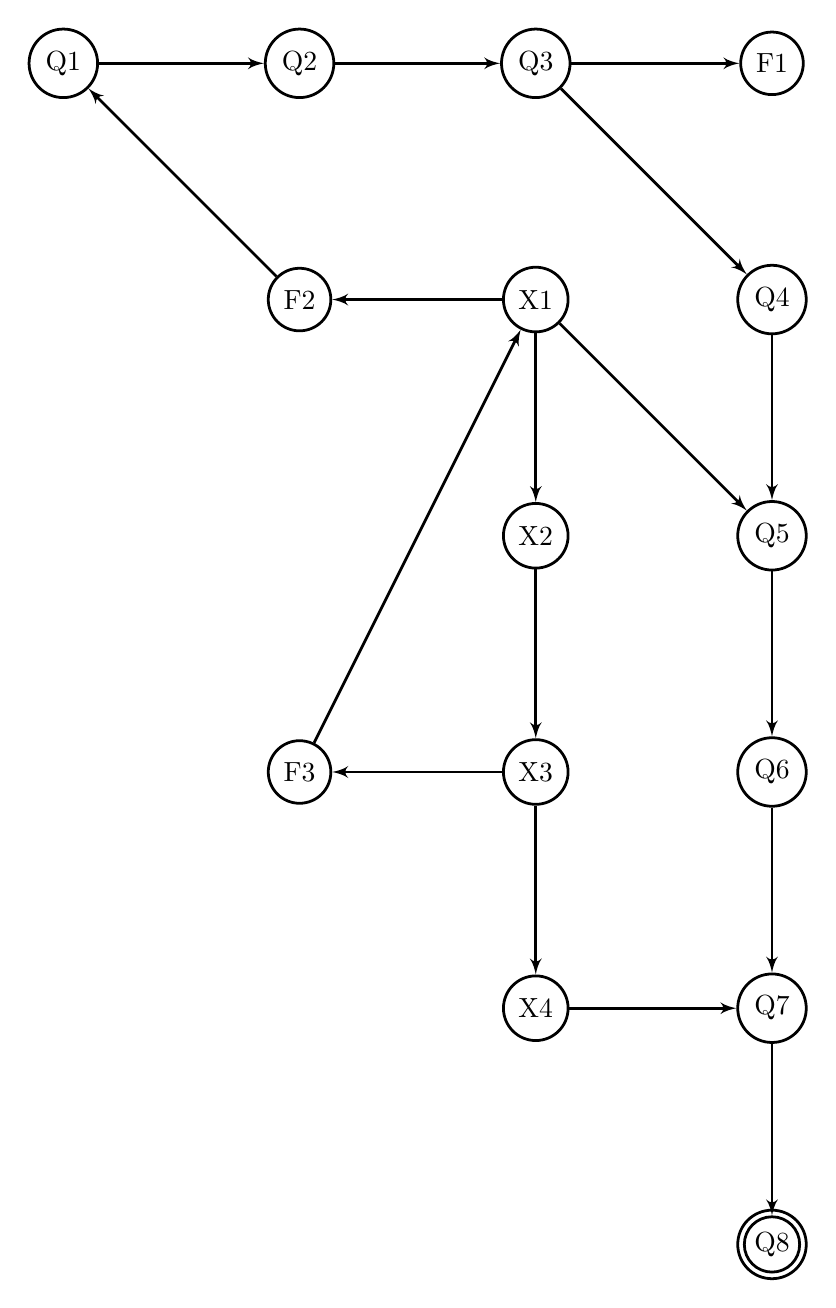
\begin{tikzpicture}[node distance = 6cm, auto, line width=1pt,>=latex]
    % Place nodes
    \node [cloud] (Q1) {Q1};
    \node [cloud, right of=Q1] (Q2) {Q2};
    \node [cloud, right of=Q2] (Q3) {Q3};
    \node [cloud, right of=Q3] (f1) {F1};
    \node [cloud, below of=f1] (Q4) {Q4};
    \node [cloud, below of=Q4] (Q5) {Q5};
    \node [cloud, below of=Q5] (Q6) {Q6};
    \node [cloud, below of=Q6] (Q7) {Q7};
    \node [cloud, below of=Q7] (Q8) {Q8};
    \node [cloud, left of=Q4] (x1) {X1};
    \node [cloud, left of=x1] (f2) {F2};
    \node [cloud, left of=Q5] (x2) {X2};
    \node [cloud, left of=Q6] (x3) {X3};
    \node [cloud, left of=x3] (f3) {F3};
    \node [cloud, left of=Q7] (x4) {X4};
    \node [cloud, below of=Q7] (Q8) {};
    % Draw edges
    \path [line] (Q1) -- (Q2);
    \path [line] (Q2) -- (Q3);
    \path [line] (Q3) -- (Q4);
    \path [line] (Q3) -- (f1);
    \path [line] (Q4) -- (Q5);
    \path [line] (x1) -- (f2);
    \path [line] (x3) -- (f3);
    \path [line] (Q5) -- (Q6);
    \path [line] (Q6) -- (Q7);
    \path [line] (Q7) -- (Q8);
    \path [line] (x1) -- (x2);
    \path [line] (x2) -- (x3);
    \path [line] (x3) -- (x4);
    \path [line] (x1) -- (Q5);
    \path [line] (x4) -- (Q7);
    \path [line] (f2) -- (Q1);
    \path [line] (f3) -- (x1);

    \end{tikzpicture}

  \newpage

\section{SYSTEM IMPLEMENTATION PLAN}

\begin{table}[ht]
\caption{System Implementation Plan Phase-I}
\vspace{1em}
\begin{tabular}{ |p{2cm}|p{7cm}|p{2.5cm}|p{3.2cm}|  }
 \hline
 \textbf{SR. NO.} & \textbf{TASK NAME} & \textbf{DURATION} & \textbf{COMPLETION}\\
 \hline
 


  1. & Project Topic Selection &  12 days & $\checkmark$\\
  \hline
  2. & Literature Survey&  15 days& $\checkmark$\\
  \hline
  3. & Study Of Existing System  &  10 days & $\checkmark$\\
  \hline
  4. & Synopsis \& Abstract Submission  &  15 days & $\checkmark$\\
  \hline
   5. & SRS   &  15 days & $\checkmark$\\
   \hline
   6. & Design Of System Architecture &  8 days & $\checkmark$\\
  \hline
  7. & Design Of UML Diagrams  &  3 days & $\checkmark$\\
  \hline
    8. & Planning Of System Modules \& Interface &  10 days & $\checkmark$\\
  \hline
 
  
  
 
 \end{tabular}
 
\end{table}

\begin{table}[ht]
\caption{System Implementation Plan Phase-II}
\vspace{1em}
\begin{tabular}{ |p{2cm}|p{7cm}|p{2.5cm}|p{3.2cm}|  }
 \hline
 \textbf{SR. NO.} & \textbf{TASK NAME} & \textbf{DURATION} & \textbf{COMPLETION}\\
 \hline
 
 9.& Implementation Of Neo-pixels ring \& Servo motor  &	10 Days	& \\
 \hline
 
10. &Implementation Of nRF24L01 Transciever &	5 Days	&\\
\hline

11. &Implementation Of IoT box	& 7 Days& \\
\hline	
12.&Implementation Of Jasper voice assistant	& 12 Days & \\
\hline
13. & Get desired output &	10 Days	& \\
\hline
14. & Testing Of Above Modules After Completion of Each Module &	3 Days Per Module	& \\
\hline
15. & Project Review &	5 Days & \\
\hline
 \end{tabular}
 
\end{table}


%%%%%%%%%%%%%%%%%%%% CHAPTER 4 %%%%%%%%%%%%%%%%%%%%%

\chapter{SYSTEM DESIGN}

\section{SYSTEM ARCHITECTURE}
The overall system design consists of following modules:
\begin{enumerate}
\item Data collection in the form of speech.
\item Voice analysis and conversion to text
\item Data storage and processing
\item Generating speech from the processed text output
\end{enumerate}

    \begin{figure}[H]
	\includegraphics[scale=0.57]{systemarchitecture.png}\\
	\caption{System Architecture}
	\end{figure}

\noindent	
System architecture consists of 4 phases, namely; Data collection in the form of voice, voice analysis and conversion to text, data storage and processing, and generating speech from the processed text output. Now, in  Data collection in the form of voice, the data is stored as input for next step. \\

\noindent
In IoT box, tasks are divided in three modules and data transmission takes place through nRF24L01 transceiver. Task modules used in IoT box are 
\begin{itemize}
\item Servo Motor for mechanical movement for object, in our case: Curtains.
\item Switching on and off Neo-pixel ring.
\item LED display : Displays the data.
\end{itemize}
\noindent
\begin{figure}
    \centering
    \includegraphics[scale=0.75]{IoTArch.png}
    \caption{IoT architrcture}
\end{figure}
\newpage
\noindent
Android application helps the user to share his personalized data through android application with ease from anywhere. The data transfer and processing is done through network adapter inbuilt APIs. This data generated is stored in firebase cloud storage and is available for the main system to access. All these tasks are being done in parallel to each other.\\

\noindent
All the data stored in Firebase cloud DB is accessible to main system and can be retrieved and process as per required. The need of given data is also processed in parallel to continuous fetching of data from the server.\\

\begin{figure}
    \centering
    \includegraphics[scale=0.60]{CloudArch.png}
    \caption{Firebase cloud server architecture}
\end{figure}

\noindent
The input voice is continuously processed and converted to text using STT along with the identifying and processing the commands using Python Script in background. The output then generated is converted from simple text to speech using TTS.\\\\
	
\section{UML DIAGRAMS}

\section{DEFINITION}
\hspace*{3em}The Unified Modelling Language (UML) is a general purpose,developmental, modelling language in the field of software
engineering, that is intended to provide a standard way to visualize the design of a system. UML was originally motivated by the desire to standardize the disparate notational systems and approaches to software design.


\section{DESIGN}
\hspace{3em}
The Unified Modelling Language (UML) offers a way to visualize a system's architectural blueprints in a diagram  including elements such as:
\begin{itemize}
\item Any activities.
\item Individual components of the system:
And how they can interact with other software components.
\item How the system will run.
\item How entities interact with others (components and interfaces)
\item External user interface
\end{itemize}

\noindent
Although originally intended solely for object oriented design documentation, the Unified Modelling Language (UML) has been extended to cover a larger set of design documentation.


\section{UML SYSTEM MODEL}
\begin{itemize}
\item \textbf{Static (or structural) view:}\\
Emphasizes the static structure of the system using objects, attributes,
operations and relationships. The structural view includes class diagrams and composite structure
diagrams.
\item \textbf{Dynamic (or behavioural) view:}\\
Emphasizes the dynamic behaviour of the system by showing collaborations among objects and changes to the internal states of objects. This view includes sequence diagrams, activity diagrams and state machine diagrams.
\end{itemize}

\section{UML MODELS}
\begin{enumerate}
\item \textbf{Use case diagram:}\\
To model a system, the most important aspect is to capture the dynamic behaviour of the system. Hence, use case diagrams are used for designing of the Dynamic nature of the system i.e. nature of the system when it is operating. Use case diagrams consists of actors, use cases and their relationships.\\
\newline
\textbf{The purposes of use case diagrams can be as follows:}
\begin{itemize}
	\item Used to gather requirements of a system.
	\item Used to get an outside view of a system.
	\item Identify external and internal factors influencing the system.
	\item Show the interacting among the requirements and actors.
\end{itemize}
\textbf{Places where use case diagrams are used:}
\begin{itemize}
	\item Requirement analysis and high level design.
	\item Model the context of a system.
	\item Reverse engineering.
	\item Forward engineering.
\end{itemize}

\item \textbf{Deployment Diagram:}\\
Deployment diagrams are used to picture the topology of the physical components i.e. Hardware components of a system where the software components are deployed. Hence, deployment diagrams are used to sketch the static deployment view of a system. It consists of nodes and their relationships.\\
\newline
\textbf{The purpose of deployment diagrams can be described as:}
\begin{itemize}
	\item Visualize hardware topology of a system.
	\item Describe the hardware components used to deploy software components.
	\item Describe run-time processing nodes.
\end{itemize}

\textbf{Usage of deployment diagrams can be described as follows:}
\begin{itemize}
	\item To model the hardware topology of a system.
	\item To model embedded system.
	\item To model hardware details for a client/server system.
	\item To model hardware details of a distributed application.
	\item Forward and reverse engineering.
\end{itemize}

\item \textbf{Activity Diagram:}\\
Activity diagram is a flow chart to represent the flow of one activity to another activity i.e. an operation of the system. So the control flow is drawn from one operation to another. This flow can be sequential, branched or concurrent. Activity diagrams deals with all type of flow control by using different elements like fork, join etc.\\
\newline
\textbf{So the purposes can be described as:}
\begin{itemize}
	\item Draw the activity flow of a system.
	\item Describe the sequence from one activity to another.
	\item Describe the parallel, branched and concurrent flow of the system.
\end{itemize}
\textbf{Following are the main usages of activity diagram:}
\begin{itemize}
	\item Modelling work flow by using activities.
	\item Modelling business requirements.
	\item High level understanding of the system's functionality.
	\item Investigate business requirements at a later stage.
\end{itemize}

\item \textbf{Sequence Diagram:}\\
The sequence diagram is used to describe some type of interactions among the different elements in the model. So this interaction is a part of dynamic behaviour of the system. Sequence diagram emphasizes on time sequence of data flow across the system.\\
\newline
\textbf{Purposes of sequence diagram can be described as:}
\begin{itemize}
    \item To capture dynamic behaviour of a system.
	\item To describe the message flow in the system.
	\item To describe structural organization of the objects.
	\item To describe interaction among objects.
\end{itemize}
	
\textbf{Following are the usages of sequence diagrams:}
\begin{itemize}
	\item To model flow of control by time sequence.
	\item To model flow of control by structural organizations.
	\item For forward engineering.
	\item For reverse engineering.
\end{itemize}

\item \textbf{State Chart Diagram:}\\
The name itself clarifies the purpose of the diagram and other details. It describes different states of a component in a system. The states are specific to a component/object of a system. A State-chart diagram describes a state machine. state machine can be defined as a machine which defines different states of an object and these states are controlled by external or internal events.\\
\newline
\textbf{Following are the main purposes of using State-chart diagrams:}
\begin{itemize}
	\item To model dynamic aspect of a system.
	\item To model life time of a reactive system.
	\item To describe different states of an object during its life time.
	\item Define a state machine to model states of an object.
\end{itemize}

\textbf{The main usages of state-chart diagrams are as follows:}
\begin{itemize}
	\item To model object states of a system.
	\item To model reactive system. Reactive system consists of reactive objects.
    \item To identify events responsible for state changes.
	\item Forward and reverse engineering.
\end{itemize}


\item \textbf{Class Diagram:}\\
The class diagram is a static diagram. It represents the static view of an application. Class diagram is used for visualizing, describing, documenting different aspects of a system and for constructing executable code of the software application. The class diagram shows a collection of classes, interfaces, associations, collaborations and constraints. It is also known as a structural diagram.\\
\newline
\textbf{Purpose of the class diagram can be summarized as:}
\begin{itemize}
	\item Analysis and design of the static view of an application.
	\item Describe responsibilities of a system.
	\item Base for component and deployment diagrams.
	\item Forward and reverse engineering.
\end{itemize}

\textbf{Class diagrams are used for:}
 \begin{itemize}
	\item Describing the static view of the system.
	\item Showing the collaboration among the elements of the static view.
	\item Describing the functionality performed by the system.
	\item Construction of software applications using object oriented languages.
\end{itemize}

\end{enumerate}

\pagebreak
    \subsection{USE CASE DIAGRAM}
    \begin{figure}[H]
    \centering
  \includegraphics[scale=0.75]{UseCase.JPG}\\
  \caption{Use Case Diagram}
  \end{figure}
    \pagebreak
    
        \subsection{CLASS DIAGRAM}
    \begin{figure}[H]
    \centering
  \includegraphics[scale=0.75]{Class.JPG}\\
  \caption{Class Diagram}
\end{figure}

    \subsection{ACTIVITY DIAGRAM}
    \begin{figure}[H]
  \centering
  \includegraphics[scale=0.75]{Activity.JPG}\\
  \caption{Activity Diagram}
\end{figure}
   \pagebreak 
   
    \subsection{DEPLOYMENT DIAGRAM}
     \begin{figure}[H]
  \centering
  \includegraphics[scale=0.75]{Deployment.JPG}\\
  \caption{Deployment Diagram}
  \end{figure}
  \pagebreak
    
    \subsection{SEQUENCE DIAGRAM}
    \begin{figure}[H]
  \centering
  \includegraphics[scale=0.65]{Sequence.JPG}\\
  \caption{Sequence Diagram}
\end{figure}
 \pagebreak   
 
    \subsection{STATE CHART DIAGRAM}
    \begin{figure}[H]
  \centering
  \includegraphics[scale=0.7]{StateChart.JPG}\\
  \caption{State Chart Diagram}
\end{figure}
\pagebreak
%%%%%%%%%%%%%%%%%% CHAPTER 5 %%%%%%%%%%%%%%%%%%%%%%
\chapter{TECHNICAL SPECIFICATION}
\section{ADVANTAGES}
\begin{itemize}
\item User Friendly interface.
\item Hands-free experience to interact between humans and computers.
\item It is portable and easy to use.
\item Connectivity with multiple devices.
\item Good interface and accessibility.
\end{itemize}

 \section{DISADVANTAGES}
     \begin{itemize}
     \item Primary disadvantage is that it is network dependent since it uses API's from different providers to fetch information.
     \item It works only with English language.
     \item One of the constraints is background noise in fetching commands through voice.
     \item Data flow is unidirectional as Firebase cloud server only sends the data and does not receive any type of data.
     \item The device is not designed for a particular voice and hence it can be less secure since anyone can use it.
     \end{itemize}
     \pagebreak
 \section{APPLICATIONS}
\begin{itemize}
\item Source of entertainment and information for blind/visually impaired.
\item Voice based calculator can be used to teach visually impaired students or it can be a game for visually sound students. 
\item Voice based spell corrector.
\end{itemize}

%%%%%%%%%%%%%%%%%% CHAPTER 6 %%%%%%%%%%%%%%%%%%%%%%%
\chapter{RESULTS}
\section{EXPECTED RESULTS}
\hspace*{3em}The project system is supposed to have voice commands as inputs, voice analyser that converts the speech to text, a processor that analyses this text based commands and generate output as the required action performed. There should be minimum noise in the input so as to avoid any error and make the system more efficient hence must have good noise cancellation. The speech to text engine is expected to work in English robustly. The system should respond to user’s request every time and in case of failure, should report the same. The android application should let the user add data such as calendar entries, set alarm, or even reminders. This data should be sent over to system cloud server and help the system keep records by using both input medium. The system should be able to implement home automation using IoT devices.

\chapter{CONCLUSION}
\noindent
The developed system will have the following phases:
\begin{itemize}
\item Data collection in the form of voice
\item Voice analysis and conversion to text
\item Data storage and processing
\item Generating speech from the processed text output.
\end{itemize}
The data generated at every phase can further be used to find patterns and suggest user later. This can be a major base for artificial intelligence machines that learns and understand users.\\
\noindent
Thus, on the basis of literature survey and by analysing the existing system, we have come to a conclusion that the proposed system will not only ease to interact with the other systems and modules but also keeps us organised.

\renewcommand{\bibname}{REFERENCES}
\begin{thebibliography}{11}
\bibitem{DE} Douglas O’Shaughnessy, Senior Member, IEEE\\
\textit{Interacting With Computers by Voice: Automatic Speech Recognition and Synthesis}

 
\bibitem {} Kei Hashimoto, Junichi Yamagishi, William Byrne, Simon King, Keiichi Tokuda
\textit{Analysis Of Machine Translation Aand Speech Synthesis In Speech-To-Speech Translation System}\\
Nagoya Institute of Technology, Department of Computer Science and Engineering, Japan\\ University of Edinburgh, Centre for Speech Technology Research, United Kingdom\\
Cambridge University, Engineering Department, United Kingdom, ISSN 5108-5111

\bibitem {} Nil Goksel-Canbek ,Mehmet Emin Mutlu\\
\textit{On the track of Artificial Intelligence: Learning with  Intelligent Personal Assistants}\\ 
ISSN:1303-5134

\bibitem{} Harshita Phatnani, Mr. Jyotiprakash Patra and Ankit Sharma\\
 \textit{Chatbot Assisting: Siri}\\ 
 E-ISSN2249–8974 

\bibitem {} Harshita Phatnani, Mr. Jyotiprakash Patra, Ankit Sharma\\
\textit{An Intelligent Voice Assistant Using Android Platform}

\bibitem {} Vinay Sagar, Kusuma SM\\
\textit{Home Automation Using IOT}\\ 
 ISSN 2395-0056.

\bibitem{} Prof Gokilavani R, Navaneethan S\\
\textit{Raspberry Pi Based Robot With Cloud Technology}\\ 
 ISSN 2321 3361

\bibitem{} Cheah Wai Zhao, Jayanand Jegatheesan, Son Chee Loon\\
\textit{Exploring IOT Application Using Raspberry Pi}

\bibitem{} Abhimanyu Chopra, Abhinav Prashar, Chandresh Sain \\
\textit{Natural Language Processing}\\
ISSN 2347-4289

\bibitem{} G. Hemalatha, C.P. Sumathi\\
\textit{A Study Of Techniques For Facial Detection and Expression Classification}
\end{thebibliography}

\newpage
\appendix
\chapter{GLOSSARY}
\begin{table}[ht]
\centering
\begin{tabular}{ |M{3cm}|p{8cm}|  }
 \hline
\textbf{NCRB}& National Crime Record Bureau \\
\hline
\textbf{SCRBx} &State Crime Record Bureaux\\
\hline
\textbf{DCRBx}&  District Crime Record Bureaux\\
\hline
\textbf{G2G} & Government to Government\\
\hline
\textbf{CCIS} & Crime Criminal Information System\\
\hline
\textbf{CIPA} & Common Integrated Police Application\\
\hline
\textbf{CBNBA} & Context Based Naive Bayesian and Apriori \\
\hline
\textbf{API} & Application Programming Interface\\
\hline
\textbf{JDK} & Java Development Kit\\
\hline
\textbf{GUI} & Graphical User Interface\\
\hline
\textbf{ID3} & Iterative Dichotomiser\\
\hline
\textbf{UML} & Unified Modelling Language\\
\hline
\textbf{DB}&  DataBase\\
\hline


\end{tabular}

\end{table}



\chapter{ASSIGNMENTS}
\section*{\centering\LARGE{LAB ASSIGNMENT 01}}

\subsection*{\underline{Aim}}
Refer Chapter 7 of first reference to develop the problem under consideration and justify feasibility using concepts of knowledge canvas and IDEA Matrix. 
\subsection*{\underline{Project}}
Voice Controlled Personal Assistant Device and Connecting IOT Devices \\

\begin{table}[ht]
\caption{Project Canvas}
\begin{tabular}{ |p{5cm}|p{5cm}|p{5cm}|  }
 \hline
 \textbf{Purpose} & \textbf{Goals} & \textbf{Users}\\
 \hline
To reduce the human efforts & To produce precise desired output with given minimal input and greater time-efficiency & All Age-Group Humans\\

To Connect IOT Devices in the vicinity & To interface the device with the IOT devices for home automation & Industries and Enterprises \\
 
 \hline
 \end{tabular}
 \end{table}
 
 \begin{table}

\vspace{0.5cm} 
 
\begin{tabular}{ |p{5cm}|p{5cm}|p{5cm}|  }
 \hline
 \textbf{Actions} & \textbf{Deliverables} & \textbf{Risks} \\
 \hline
 To define functionality of device along with respective vocal commands  & SRS \& Project Design & Features should work in harmony and both time and space efficiency\\


  Work on different Modules of Project to build an integrated system & Project Report \& Project & Device may not be able to perform the service according to command\\
   \hline
 
 \end{tabular}
 \end{table}
\vspace{0.5cm} 
\begin{table}
 \begin{tabular}{ |p{5cm}|p{5cm}|p{5cm}|  }
 \hline
 \textbf{Milestones} & \textbf{Constraints} & \textbf{Scope} \\
 \hline
 Synopsis, Abstract, Report & All Functionality well defined with all possible voice commands which & Commands limited to only English\\

  Coding and Final Software  & Device should work in any environment & Limited to quality of the vocal commands\\ 
   \hline
 \end{tabular}
\end{table} 
\pagebreak
\newpage
\noindent\\\\
\\\\
\\\\
\\\\
\\\\
\\\\
\\\\
\\\\
\\\\
\\\\
\\\\
\section*{\centering\LARGE{LAB ASSIGNMENT 02}}
\subsection*{\underline{Aim}}
Project problem statement feasibility assessment using NP-Hard, NP-Complete or satisfy ability issues using modern algebra and/or relevant mathematical models.

\subsection*{\underline{Feasibility Theory}}
The feasibility of the project can be defined as the measure of our project whether it is viable or not.It includes various different types of feasibility as follows:
\begin{itemize}
\item \textbf{Performance:}\\
In this we check whether the proposed system is capable of performing all the functional requirements as mentioned in system features in SRS.If our system is performing the functional requirements appropriately then it's performance is feasible.Here we also check the accuracy and efficiency of the system based on various STT-TTS Engines.
\item \textbf{Technical:}\\
In this we check whether the technical specification provided that is hardware and software requirements are minimum requirements for our platform to run successfully without any error regarding the system configuration. Also the voice commands are suffice to call a predefined functionality module and features are performed effectively.
\item \textbf{Economical:}\\
In this we check the cost per line of code, also the cost for storage of hardware required and cost related to the run time of the system.Apart from this since no large database transactions are needed apart from minimum system data which will be required for profilication.

\end{itemize}
\noindent
\subsection*{\underline{Feasibility on basis of Class of Problem}}
\hspace{3em}Complexity classes are one way to talk about how difficult or easy a problem is.
Complexity theory gets very technical but the basics are actually extraordinarily
intuitive, and it's possible to understand the P versus NP issue with very little
math background.\\

\noindent
If there is a fast solution to the search version of a problem then the problem is
said to be Polynomial time, or P for short. If there is a fast solution to the verification version of a problem then the problem is said to be Non deterministic Polynomial time,
or NP for short. The question of "P=NP" is then the question of whether these sets are identical.\\

\noindent
Some problems can be translated into one another in such a way that a fast
solution to one problem would automatically give us a fast solution to the
other. There are some problems that every single problem in NP can be
translated into, and a fast solution to such a problem would automatically give
us a fast solution to every problem in NP. This group of problems are known as
NP Hard.Some problems in NP Hard
are actually not themselves in NP; the
group of problems that are in both NP and NP Hard
is called NP Complete

\subsection*{\underline{Classes of problems}}
\begin{itemize}
\item \textbf{NP}\\
A lot of programs that don't (necessarily) run in polynomial time
on a regular computer, but do run in polynomial time on a non deterministic
Turing machine. These programs solve problems in NP, which stands for
non deterministic polynomial time.An equivalent way to define NP is by pointing to the problems that can be
verified in polynomial time.

\item \textbf{NP Hard}\\
If a problem is NP hard,
this means I can reduce any problem in NP to that problem. This means if I can solve that problem, I can easily solve any problem in NP. If we could solve an NP hard
problem in polynomial time, this would
prove P = NP.

\item \textbf{NP Complete}\\
A problem is NP complete
if the problem is both
NP hard, and in NP.
\end{itemize}

\noindent
\hspace{3em}Our system satisfies not only problems of bringing different services under one platform as well as we are adding many functionality which are not provided by other personal assistant devices and connecting IOT devices as well as extending usability by providing and Android application as well.\\

\noindent
\hspace{3em}Since we have a fast solution to convert the speech into a recognizable functionality it is said to be P type problem capable to solve a part in polynomial time also the servicing the functionality doesn't has a fast solution so it  is not a NP complete problem.
\subsection*{\underline{Relation Between Classes of Problems}}
 \begin{figure}[H]
    \centering
  \includegraphics[scale=0.9]{nprelation.PNG}\\
  \caption{Relation between Classes of Problems}

\end{figure}
     \subsection*{\underline{Mathematical Model}}
  \textbf{Mathematical Formulation:}\\
Let the M i the universal states which contains, \\
    \textbf{M = \{Q, S, F, Q1 , Qf \}} \newline
    where, \\
    \newline
    		Q = No. of states \{Q1,Q2,Q3,Q4,Q5,Q6,Q7,Q8\}\\
    		X = No. of states \{X1, X2, X3, X4\}\\
    		Q1 = Initial State.\\
    		S = Success state.\\
    		F = Failure state.\\
    		\newline
    where,\\ 
    \newline
    Q1= Start.\\
     \newline
    Q2 = Initialize assistant by calling action word. \\
    \newline
    Q3 = Once initialized, give input in the speech format.\\
    \newline
    Q4 = Processing of speech into text.\\
    \newline 
    Q5 = Text is compared with commands.\\
    \newline
    Q6 = Perform action according to command.\\
    \newline 
    Q7 = Convert the action into speech.\\
    \newline 
    Q8 = Give output in the speech format.\\
    \newline
    X1 = Connect Personal AI Device to mobile application.\\
    \newline
    X2 = Update To-Do list, Calender, Alarm, reminder, etc.\\
    \newline
    X3 = Updated data is sent to cloud server.\\
    \newline
    X4 = According to the data sent, AI Device will take action.\\
    \newline

\noindent   
\textbf{Failure Conditions:}  F = \{F1,F2,F3\} \newline
\begin{itemize}
\item F1  = Failure if the device is not initialised due to noisy background.
\item F2 = Connection with android app failed.
\item F3 = Server down failure or cannot retrieve data from server.
\end{itemize}

\noindent
 \textbf{Success Conditions:} S = \{S1\}
    \begin{itemize}
    		\item S1 = Success after the data is assimilated and output is produced accordingly.
	\end{itemize}     

\subsection*{\underline{Activity Diagram}}
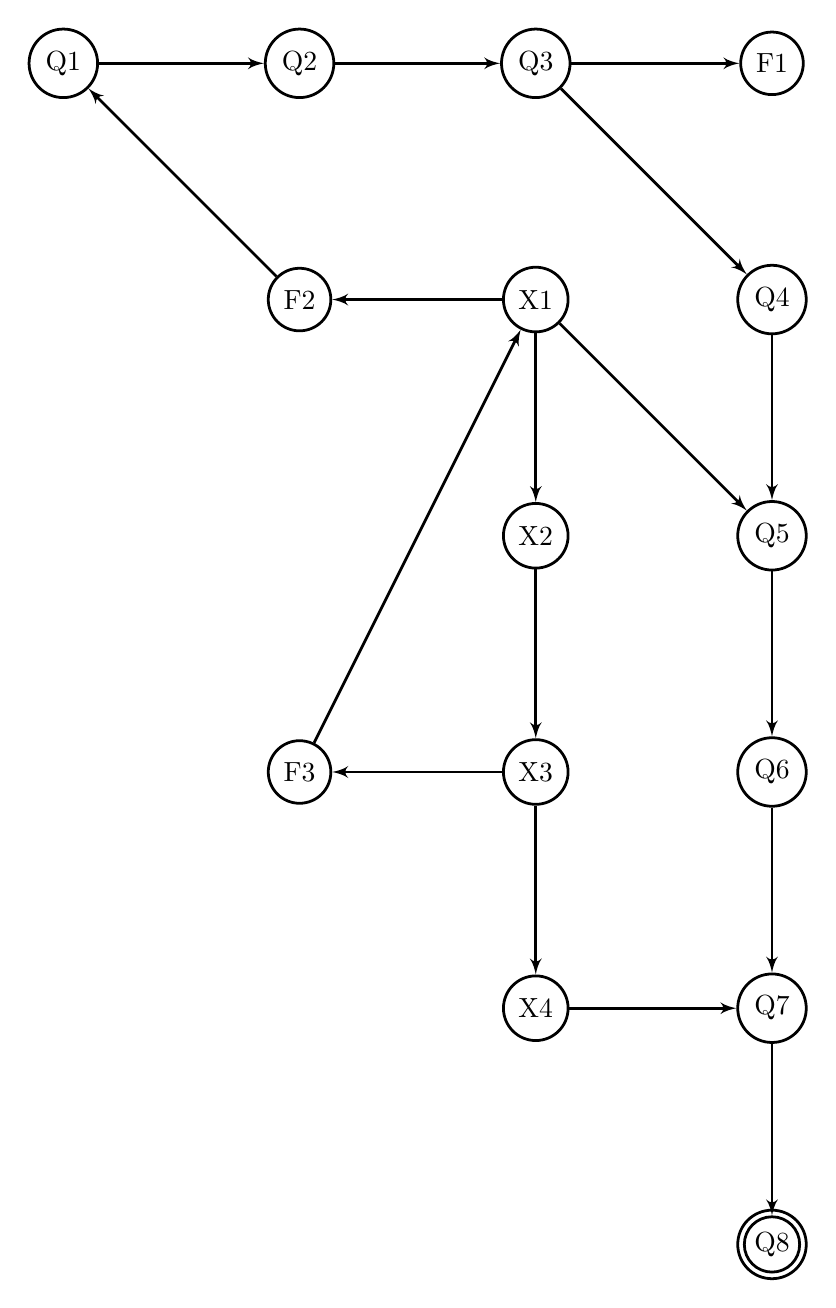
\begin{tikzpicture}[node distance = 6cm, auto, line width=1pt,>=latex]
    % Place nodes
    \node [cloud] (Q1) {Q1};
    \node [cloud, right of=Q1] (Q2) {Q2};
    \node [cloud, right of=Q2] (Q3) {Q3};
    \node [cloud, right of=Q3] (f1) {F1};
    \node [cloud, below of=f1] (Q4) {Q4};
    \node [cloud, below of=Q4] (Q5) {Q5};
    \node [cloud, below of=Q5] (Q6) {Q6};
    \node [cloud, below of=Q6] (Q7) {Q7};
    \node [cloud, below of=Q7] (Q8) {Q8};
    \node [cloud, left of=Q4] (x1) {X1};
    \node [cloud, left of=x1] (f2) {F2};
    \node [cloud, left of=Q5] (x2) {X2};
    \node [cloud, left of=Q6] (x3) {X3};
    \node [cloud, left of=x3] (f3) {F3};
    \node [cloud, left of=Q7] (x4) {X4};
    \node [cloud, below of=Q7] (Q8) {};
    % Draw edges
    \path [line] (Q1) -- (Q2);
    \path [line] (Q2) -- (Q3);
    \path [line] (Q3) -- (Q4);
    \path [line] (Q3) -- (f1);
    \path [line] (Q4) -- (Q5);
    \path [line] (x1) -- (f2);
    \path [line] (x3) -- (f3);
    \path [line] (Q5) -- (Q6);
    \path [line] (Q6) -- (Q7);
    \path [line] (Q7) -- (Q8);
    \path [line] (x1) -- (x2);
    \path [line] (x2) -- (x3);
    \path [line] (x3) -- (x4);
    \path [line] (x1) -- (Q5);
    \path [line] (x4) -- (Q7);
    \path [line] (f2) -- (Q1);
    \path [line] (f3) -- (x1);

    \end{tikzpicture}


\newpage
\section*{\centering\LARGE{Lab Assignment 03}}
\subsection*{\underline{Aim}}
\noindent
Use of divide and conquer strategies to exploit distributed/parallel/concurrent processing of the above to identify objects, morphisms, overloading in functions (if any), and functional relations and any other dependencies (as per requirements).
\subsection*{\underline{Concept}}
\hspace*{3em}A divide and conquer algorithm works by recursively breaking down a problem into two or more sub-problems of the same (or related) type (divide), until these become simple enough to be solved directly (conquer). So have divided our problem based on modules used and those are:
\begin{itemize}
\item IOT box
\item Android Smart-phone application
\item Voice input and processing.
\item Get data from Firebase cloud DB.
\item Generating speech using TTS task model.
\end{itemize}

\noindent
Divide and conquer (D\&C) is an algorithm design paradigm based on multi-branched recursion. So we have to recursively divide our problem into  sub-problems  of the same (or related) type (divide), until these sub-problem become simple enough to be solved directly (conquer). The solutions to the sub-problems are then combined to give a solution to the original problem.\\

\noindent
In our project we have divided our project into 4 phases which are : Data collection in the form of voice, voice analysis and conversion to text, data storage and processing, and generating speech from the processed text output. Now, in  Data collection in the form of voice, the data is stored as input for next step. \\

\noindent
In IoT box, tasks are divided in three modules and data transmission takes place through nRF24L01 transceiver. Task modules used in IoT box are 
\begin{itemize}
\item Servo Motor for mechanical movement for object, in our case: Curtains.
\item Switching on and off Neo-pixel ring.
\item LED display : Displays the data.
\end{itemize}

\noindent
Android application helps the user to share his personalized data through android application with ease from anywhere. The data transfer and processing is done through network adapter inbuilt APIs. This data generated is stored in firebase cloud storage and is available for the main system to access. All these tasks are being done in parallel to each other.\\

\noindent
All the data stored in Firebase cloud server is accessible to main system and can be retrieved and process as per required. The need of given data is also processed in parallel to continuous fetching of data from the server.\\

\noindent
The input voice is continuously processed and converted to text using STT along with the identifying and processing the commands using Python Script in background. The output then generated is converted from simple text to speech using TTS.\\
     
    \begin{figure}[H]
    \includegraphics[scale=0.60]{sysflow.png}\\
    \caption{Data-flow Diagram}
    \end{figure}

\newpage
\section*{\centering\LARGE{Lab Assignment 04}}
\subsection*{\underline{Aim}}
Use of above to draw functional dependency graphs and relevant Software modelling methods, techniques including UML diagrams or other necessities using appropriate tools.
    \subsection*{USE CASE DIAGRAM}
    \begin{figure}[H]
    \centering
  \includegraphics[scale=0.75]{UseCase.JPG}\\
  \caption{Use Case Diagram}
  \end{figure}
    \pagebreak
    
        \subsection*{CLASS DIAGRAM}
    \begin{figure}[H]
    \centering
  \includegraphics[scale=0.75]{Class.JPG}\\
  \caption{Class Diagram}
\end{figure}

    \subsection*{ACTIVITY DIAGRAM}
    \begin{figure}[H]
  \centering
  \includegraphics[scale=0.75]{Activity.JPG}\\
  \caption{Activity Diagram}
\end{figure}
   \pagebreak 
   
    \subsection*{DEPLOYMENT DIAGRAM}
     \begin{figure}[H]
  \centering
  \includegraphics[scale=0.75]{Deployment.JPG}\\
  \caption{Deployment Diagram}
  \end{figure}
  \pagebreak
    
    \subsection*{SEQUENCE DIAGRAM}
    \begin{figure}[H]
  \centering
  \includegraphics[scale=0.65]{Sequence.JPG}\\
  \caption{Sequence Diagram}
\end{figure}
 \pagebreak   
 
    \subsection*{STATE CHART DIAGRAM}
    \begin{figure}[H]
  \centering
  \includegraphics[scale=0.7]{StateChart.JPG}\\
  \caption{State Chart Diagram}
\end{figure}
\pagebreak

\newpage
\section*{\centering\LARGE{Lab Assignment 05}}
\subsection*{\underline{Aim}}
Testing of project problem statement using generated test data (using mathematical models, GUI, Function testing principles, if any) selection and appropriate use of testing tools, testing of UML diagram's reliability.
\noindent
\subsection*{\underline{Testing}}
\textbf{WHAT IS SOFTWARE TESTING?}\\
\hspace{5em} Software testing is a process of verifying and validating that a software application or program\\
1. Meets the business and technical requirements that guided its design and development, and\\
2. Works as expected.\\\\
Software testing also identifies important defects, flaws, or errors in the application code that must be fixed.\\
\newline
\noindent
\hspace{5em}Software testing has three main purposes: verification, validation, and defect finding.
\begin{itemize}
 \item The verification process confirms that the software meets its technical specifications. A “specification” is a
description of a function in terms of a measurable output value given a specific input value under specific
preconditions. A simple specification may be along the line of “a SQL query retrieving data for a single
account against the multi-month account-summary table must return these eight fields $<$list$>$ ordered by
month within 3 seconds of submission.”
 \item The validation process confirms that the software meets the business requirements. A simple example of a
business requirement is “After choosing a branch office name, information about the branch’s customer account managers will appear in a new window. The window will present manager identification and summary information about each manager’s customer base: $<$list of data elements$>$.” Other requirements
provide details on how the data will be summarized, formatted and displayed.
 \item A defect is a variance between the expected and actual result. The defect’s ultimate source may be traced
to a fault introduced in the specification, design, or development (coding) phases. 
\end{itemize}
\newpage

\noindent
\textbf{Software testing answers questions that development testing and code reviews can’t}
\begin{enumerate}
\item Does it really work as expected?
\item Does it meet the users’ requirements?
\item Is it what the users expect?
\item Do the users like it?
\item Is it compatible with our other systems?
\item How does it perform?
\item How does it scale when more users are added?
\item Which areas need more work?
\item Is it ready for release?
\end{enumerate}
\textbf{What can we do with the answers to these questions?}
\begin{enumerate}
\item Save time and money by identifying defects early
\item Avoid or reduce development downtime
\item Provide better customer service by building a better application
\item Know that we’ve satisfied our users’ requirements
\item Build a list of desired modifications and enhancements for later versions
\item Identify and catalog reusable modules and components
\item Identify areas where programmers and developers need training 
\end{enumerate}

\subsection*{\underline{The Test Plan}}
\noindent
\hspace{3em}
The test plan is a mandatory document. You can’t test without one. For simple, straight-forward projects the plan
doesn’t have to be elaborate but it must address certain items. As identified by the “American National Standards
Institute and Institute for Electrical and Electronic Engineers Standard 829/1983 for Software Test Documentation”,
the following components should be covered in a software test plan.\\
    
\begin{table}[ht]
    \caption{Test Plan}
    \begin{tabular}{ |p{5cm}|p{5cm}|p{5cm}|  }
    \hline
    \textbf{Component} & \textbf{Description} & \textbf{Purpose}\\
    \hline
    Responsibilities & Specific people who are and their assignments & Assigns responsibilities and keeps everyone on track and focused\\\hline

    Assumptions & Code and systems status and availability & Avoids misunderstandings about schedules \\\hline
    
    Test & Testing scope,schedule,duration, and prioritization & Outlines the entire process and maps specific tests \\\hline
    
    Communication & Communications plan-- who, what, when, how & Everyone knows what they need to know it \\\hline
    
    Risk Analysis & Critical items that will be tested & Provides focus by identifying areas that are critical for success \\\hline
    
    Defect Reporting & How defect will be logged and documented & Tells how to document a defect so that it can be reproduced, fixed, and retested \\\hline
    
    Environment & The technical environment, data, work area, and interfaces used in testing & Reduces or eliminates misunderstandings and sources of potential delay \\
 
    \hline
    \end{tabular}
\end{table}

\subsection*{\underline{Types of Software Tests}}
It describes which testing types we might follow in our testing life cycle.
    \begin{figure}[H]
        \centering
            \includegraphics[scale=0.65]{SoftwareTesting.JPG}\\
        \caption{Types of software testing}
  \end{figure}
\begin{itemize}
\item \textbf{Black Box Testing}\\
Black box testing methods focus on the functional requirements in the software. That is, black box testing enables us to derive sets of input conditions that will fully exercise.\\
All functional requirements of the program Black box testing attempts to find errors in the following categories:
\begin{itemize}
\item Incorrect or missing function
\item	Interface errors
\item	Errors in data structure or external job access
\item	Performance errors
\item	Initialization and termination errors.
 
\end{itemize}
In the proposed application with the help of this technique, we do not use the code to determine a test suite; rather, knowing the problem that we are trying to solve, we come up with four types of test data: 
\begin{enumerate}
\item	Easy-to-compute data,
\item	Typical data,
\item	Boundary / extreme data,
\item	Bogus data.

\end{enumerate}

\item \textbf{Unit Testing}\\
Unit testing enables a programmer to detect error in coding. A unit test focuses verification of the smallest unit of software design. This testing was carried out during the coding itself. In this testing step, each module going to be work satisfactorily as the expected output from the module.\\

\noindent
The front end design consists of various forms. They were tested for data acceptance. Similarly, the back-end also tested for successful acceptance and retrieval of data. The unit testing is done on the developed code. Mainly the unit testing is done on modules.

\item \textbf{System Testing}\\
After performing the integration testing, the next step is output testing of the proposed system. No system could be useful if it doesn't produce the required output in a specified format. The outputs generated are displayed by the user. Here the output format is considered in to two ways. One in on screen and other in printed format.

\item \textbf{Integration Testing}\\
Through each program work individually, they should work after linking together. This is referred to as interfacing. Data may be lost across the interface; one module can have adverse effect on the other subroutines after linking may not do the desired function expected by the main routine. Integration testing is the systematic technique for constructing the program structure while at the same time conducting test to uncover errors associated with the interface. Using integrated test plan prepared in the design phase of the system development as a guide, the integration test was carried out. All the errors found in the system were corrected for the next testing step.

\item \textbf{User Acceptance Testing}\\
User Acceptance Testing is also called Beta testing, application testing, and end-user testing. Whatever you choose
to call it, it’s where testing moves from the hands of the IT department into those of the business users. Software
vendors often make extensive use of Beta testing, some more formally than others, because they can get users to do
it for free. \\

\noindent
By the time UAT is ready to start, the IT staff has resolved in one way or another all the defects they identified.
Regardless of their best efforts, though, they probably don’t find all the flaws in the application. A general rule of
thumb is that no matter how bulletproof an application seems when it goes into UAT, a user somewhere can still find a
sequence of commands that will produce an error. \\
\item \textbf{Product verification Testing}\\
Production verification testing is a final opportunity to determine if the software is ready for release. Its purpose is to
simulate the production cut-over as closely as possible and for a period of time simulate real business activity. As a
sort of full dress rehearsal, it should identify anomalies or unexpected changes to existing processes introduced by
the new application. For mission critical applications the importance of this testing cannot be overstated.\\

\noindent
The application should be completely removed from the test environment and then completely reinstalled exactly as it
will be in the production implementation. Then mock production runs will verify that the existing business process
flows, interfaces, and batch processes continue to run correctly. Unlike parallel testing in which the old and new
systems are run side-by-side, mock processing may not provide accurate data handling results due to limitations of
the testing database or the source data. 

\begin{table}[ht]
    \caption{Black-Box Test Plan of the Platform}
    \begin{tabular}{ |p{4cm}|p{4cm}|p{3cm}|p{4cm}|  }
    \hline
    \textbf{Component} & \textbf{Description} & \textbf{Input} & \textbf{Expected Output}\\
    \hline
    Proper Recognition of Command & To check command in English is recognised by Device as correctly & Vocal Command & Command is recognised by the device \\\hline

    Android Connectivity to Cloud DB & To check that data is transfered properly in both the direction to the Firebase Cloud DB with real-time results & Android App and Firebase Cloud DB & Android Application Updates are recognised by the platform\\\hline
    
    Performance of IOT Box & To check whether IOT Box performs correctly on the input of concerned commands & IOT Box Related Vocal Commands & IOT Box Works Seamlessly\\\hline
    
    Performance of Firebase Cloud & To check whether Firebase work with no downtime, real-time services and Provide API form Device and Android application  & Firebase Cloud DB & Firebase Cloud Db works as expected with Python and Android API\\\hline
    
    Response Of AI Device & To check whether the AI Device Vocal response to commands are correct & Vocal Commands along with required parameters & Output vocal command is the correct response to the input command\\\hline
    
    Integration test of the Platform & To check whether all the modules of the platform is working properly when interfaced together as one & All the modules if the platform & Data flows throughout the platform from one end to another without any errors\\
 
    \hline
    \end{tabular}
\end{table}
\end{itemize}





%\begin{table}[ht]
%\caption{Test Cases}
%\begin{tabular}{ |M{4cm}|p{5cm}|M{2.5cm}|M{3.2cm}|  }
% \hline
 %\textbf{USE CASE} & \textbf{FUNCTION BEING TESTED} & \textbf{INPUT} & \textbf{EXPECTED OUTPUT}\\
 %\hline
 
%Data Collection & Is data collected properly? & Web data & Stored records in DB\\

%\hline
 %Data Classification & Is data classified into  classes as per attributes? & Data in DB & Classes of attributes\\
 
 %\hline
 %Pattern identification & Is unique patterns generated? & Classes from classifier & Patterns as rules.\\
 
 %\hline
 %Prediction & Is regions having a common pattern? & Rules from apriori & Expected output\\
  
  %\hline
  
 
 %\end{tabular}
 
%\end{table}
%\end{comment}


\end{document}